% !Mode:: "TeX:UTF-8"

\begin{frame}{第十九讲、坐标变换与重积分的计算}
	\linespread{1.5}
	\begin{enumerate}
	  \item {\bf 内容与要求}{\b (\S 11.3)}
	  \begin{itemize}
		\item 熟练掌握二重积分在极坐标下的计算
		\item 熟练掌握二重积分在柱坐标下的计算
		\item 熟练掌握三重积分在球坐标下的计算
% 	    \item 熟练掌握三重积分计算的微元法和截痕法
	  \vspace{1em}
	  \end{itemize}
	  \item {\bf  课后作业:}
	  \begin{itemize}
	    \item {\b 习题11.3:2(2,4),3(2)}
	    \item {\b 习题11.3:4(2),5(2),6(1,3),11(3,4),16}
	  \end{itemize}
	\end{enumerate}
\end{frame}

\section{二重积分在极坐标下的计算}

\begin{frame}{二重积分在极坐标下的计算}
	\linespread{1.2}\pause 
	{\bf 直角坐标下的二重积分:}
	$$I=\iint_Df(x,y)\d\sigma=\iint_Df(x,y)\d x\d y$$
	\pause 在极坐标系下,面积微元$\alert{\d\sigma=\rho \d\rho \d\theta}$,\pause 
	从而
	$$\alert{I=\iint_Df(x,y)\d\sigma=\iint_Df(\rho\cos\theta,\rho\sin\theta)
	\rho \d\rho \d\theta}$$
	\pause \ba{注意:微元形式的改变意味着积分区域表示方式的变化}
\end{frame}

\begin{frame}{极坐标下积分区域的表示}
	\linespread{1.2}\pause 
	\begin{columns}
		\column{.5\textwidth}
			\begin{center}
				\resizebox{!}{4.2cm}{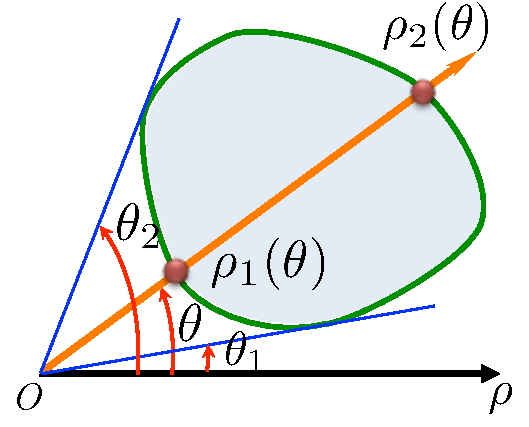
\includegraphics{./images/ch11/tr.pdf}}\pause 
			\end{center}
			$$D:\theta_1\leq\theta\leq\theta_2,$$
			$$\rho_1(\theta)\leq\rho\leq\rho_2(\theta)$$
		\column{.5\textwidth}\pause 
			\begin{center}
				\resizebox{!}{4.2cm}{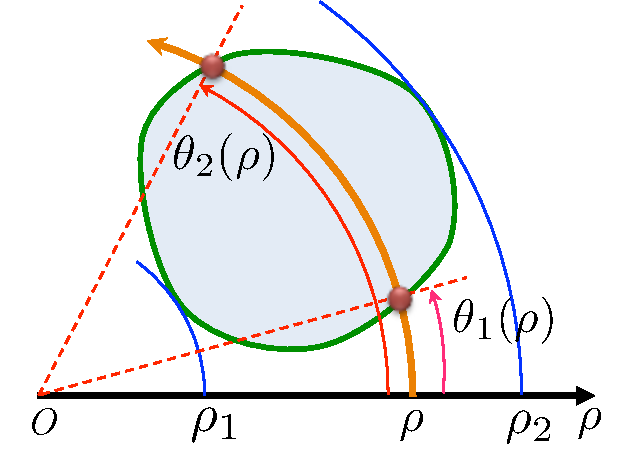
\includegraphics{./images/ch11/rt.pdf}}\pause 
			\end{center}
			$$D:\rho_1\leq\rho\leq\rho_2,$$
			$$\theta_1(\rho)\leq\theta\leq\theta_2(\rho)$$
	\end{columns}
\end{frame}

\begin{frame}
	\linespread{1.2}
	\begin{exampleblock}{{\bf 例1}\hfill}
		计算二重积分
		$$\iint_D(x^2+y^2)\d x\d y,$$
		其中$D$由圆$x^2+y^2=2y,\,x^2+y^2=4y$及直线
		$x=\sqrt 3y,\,y=\sqrt 3x$围成。
	\end{exampleblock}
\end{frame}

\begin{frame}
	\linespread{1.2}
	\begin{exampleblock}{{\bf 例2}\hfill}
		计算二重积分
		$$\iint_D\arctan\df yx\d\sigma,$$
		其中$D$为双扭线
		$$(x^2+y^2)^2=a^2(x^2-y^2)\;(a>0)$$
		与$x$轴正向围成图形在第一象限中的部分。
	\end{exampleblock}
\end{frame}

\begin{frame}
	\linespread{1.2}
	\begin{exampleblock}{{\bf 例3}\hfill}
		求球体$x^2+y^2+z^2\leq 4a^2$包含在圆柱$x^2+y^2=2ax$
		
		$\,(a>0)$
		内的体积。
	\end{exampleblock}
	\pause 
	\begin{center}
		\resizebox{!}{5cm}{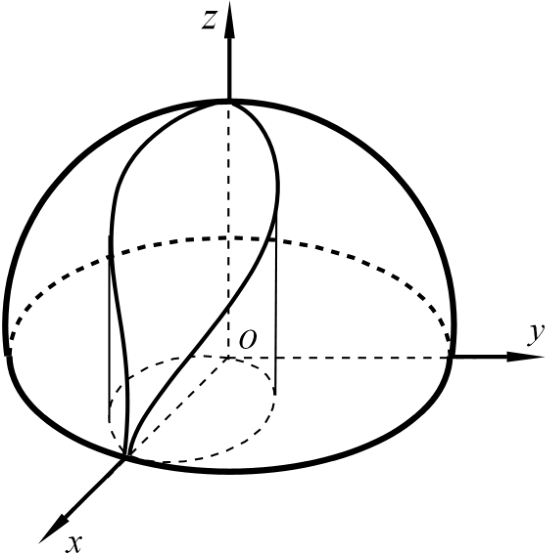
\includegraphics{./images/ch10/viviani.pdf}}
	\end{center}
\end{frame}

\begin{frame}
	\linespread{1.2}
	\begin{exampleblock}{{\bf 例4}\hfill}
		计算椭圆抛物面$z=x^2+2y^2$与抛物柱面$z=2-x^2$所围成
		的立体体积。
	\end{exampleblock}
	\pause 
	\begin{center}
		\resizebox{!}{5cm}{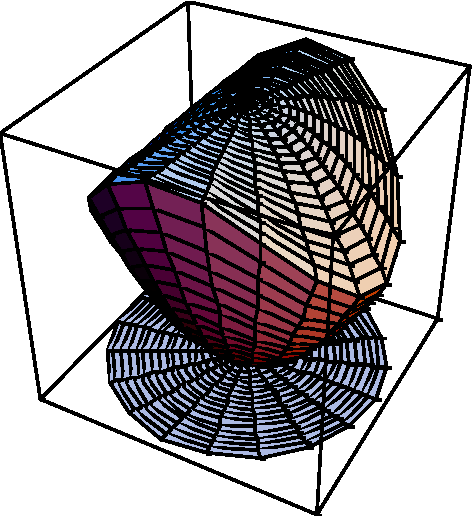
\includegraphics{./images/ch11/ub.pdf}}
	\end{center}
\end{frame}

\begin{frame}
	\linespread{1.2}
	\begin{alertblock}{{\bf 例5}\hfill}
		计算
		$$\iint_De^{-x^2-y^2}\d x\d y,$$
		其中$D:x^2+y^2\leq a^2$。利用该计算结果求
		$$\dint_{-\infty}^{+\infty}e^{-x^2}\d x.$$
	\end{alertblock}
\end{frame}

\begin{frame}[<+->]{小结}
	\linespread{1.2}
	\ba{二重积分在极坐标系下的计算}
	\begin{enumerate}
	  \item {\bf 面积微元的变化}
	  $$\d\sigma=\d x\d y=\rho \d\rho \d\theta$$
	  \item {\bf 积分区域的表示:}极坐标下的“矩形”
	  \item {\bf 特殊定积分:}
	  $$\dint_{-\infty}^{+\infty}e^{-x^2}\d x=\sqrt{\pi}$$
	\end{enumerate}
\end{frame}

\section{三重积分在柱坐标下的计算}

\begin{frame}{三重积分在柱坐标下的计算}
	\linespread{1.2}\pause 
	{\bb 柱坐标系:}\pause 
	$$M:\;(x,y,z)\;\to(\rho,\theta,z)$$
	\vspace{-2em}
	\begin{columns}\pause 
		\column{.5\textwidth}
			$$\alert{\left\{\begin{array}{l}
				x=\rho\cos\theta\\
				y=\rho\sin\theta\\
				z=z
			\end{array}\right.}$$
			\pause 其中
			$$\alert{\rho\geq 0,0\leq\theta\leq 2\pi,z\in\mathbb{R}}$$
		\column{.5\textwidth}\pause 
			\begin{center}
				\resizebox{!}{5cm}{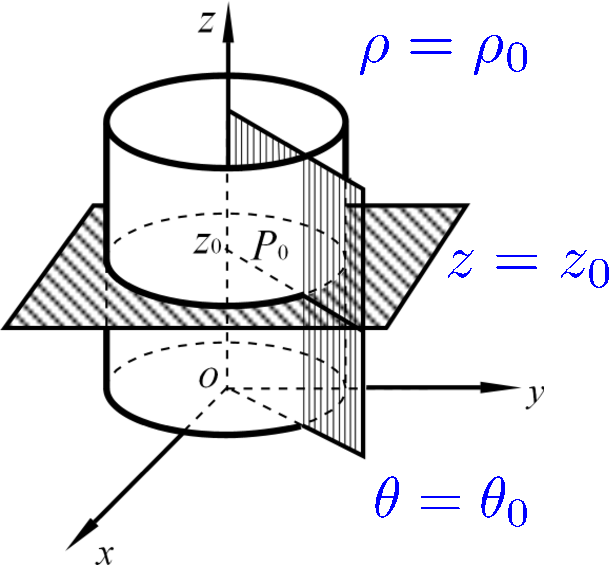
\includegraphics{./images/ch11/bucket.pdf}}
			\end{center}
	\end{columns}
\end{frame}

\begin{frame}{柱坐标系下的体积微元}
	\linespread{1.2}
	\begin{columns}\pause 
		\column{.6\textwidth}
			\begin{center}
				\resizebox{!}{5cm}{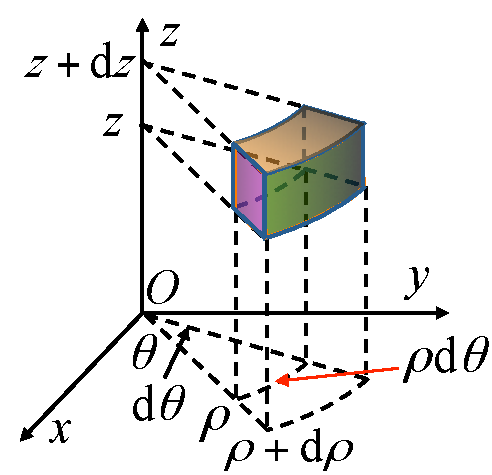
\includegraphics{./images/ch11/polarCy.pdf}}
			\end{center}
		\column{.4\textwidth}\pause 
			{\Large
			$$\alert{\d V=\rho \d\rho \d\theta \d z}$$
			}
	\end{columns}\pause 
	$$\alert{\iiint_{\Omega}f(x,y,z)\d
	V=\iiint_{\Omega}f(\rho\cos\theta,\rho\sin\theta,z)\rho \d\rho \d\theta \d z}$$
\end{frame}

\begin{frame}{柱坐标系下积分区域的表示}
	\linespread{1.2}
	\begin{columns}\pause 
		\column{.5\textwidth}
			{\bb 微元法:}\pause 
			\begin{itemize}
			  \item $\alert{\theta_1\leq\theta\leq\theta_2}$\pause 
			  \item $\alert{\rho_1(\theta)\leq\rho\leq\rho_2(\theta)}$\pause 
			  \item $\alert{z_1(\rho,\theta)\leq z\leq z_2(\rho,\theta)}$\pause 
			\end{itemize}
		\column{.5\textwidth}
			\begin{center}
				\resizebox{!}{6cm}{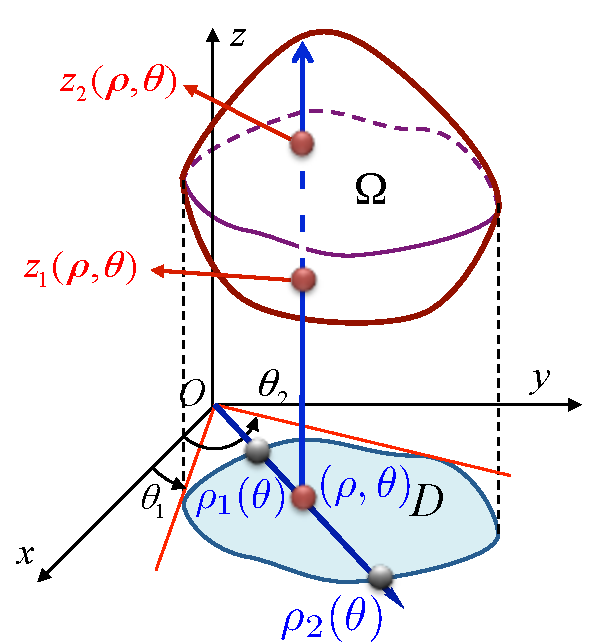
\includegraphics{./images/ch11/cy21.pdf}}
			\end{center}

	\end{columns}
\end{frame}

\begin{frame}
	\linespread{1.2}
	\begin{exampleblock}{{\bf 例6}\hfill}
		计算三重积分
		$$\iiint_{\Omega}z\sqrt{x^2+y^2}\d V,$$
		其中$\Omega$为柱面$x^2+y^2=2x\,(y>0)$与平面
		$z=0,\,$
		
		$z=h\,(h>0)$所围立体。
	\end{exampleblock}
\end{frame}

\begin{frame}
	\linespread{1.2}
	\begin{exampleblock}{{\bf 例7}\hfill}
		计算三重积分
		$$\iiint_{\Omega}\df 1{1+x^2+y^2}\d V,$$
		其中$\Omega$由$x^2+y^2=4z$与$z=h\,(h>0)$所围成。
	\end{exampleblock}
\end{frame}

\section{三重积分在球坐标下的计算}

\begin{frame}{三重积分在球坐标下的计算}
	\linespread{1.2}\pause 
	{\bb 球坐标系:}
	$$M:\;(x,y,z)\;\to(r,\theta,\varphi)$$
	\vspace{-2em}
	\begin{columns}\pause 
		\column{.5\textwidth}
			$$\alert{\left\{\begin{array}{l}
				x=r\sin\varphi\cos\theta\\
				y=r\sin\varphi\sin\theta\\
				z=r\cos\varphi
			\end{array}\right.}$$
			\pause 其中
			$$\alert{r\geq 0,0\leq\theta\leq 2\pi,0\leq\varphi\leq\pi}$$
		\column{.5\textwidth}\pause 
			\begin{center}
				\resizebox{!}{5cm}{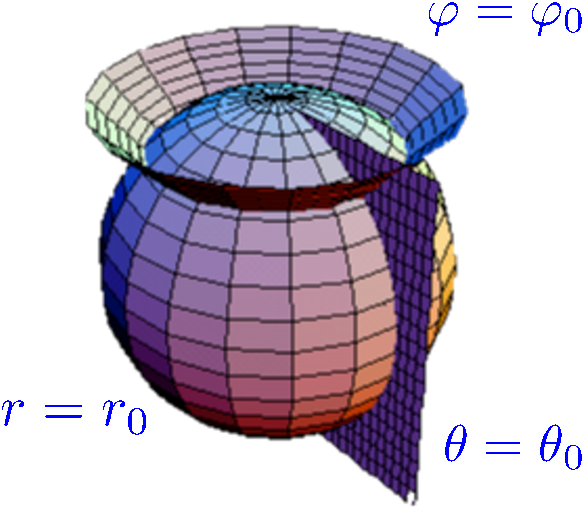
\includegraphics{./images/ch11/sphereP.pdf}}
			\end{center}
	\end{columns}
\end{frame}

\begin{frame}{球坐标系下的体积微元}
	\linespread{1.2}\pause 
% 	\begin{columns}
% 		\column{.6\textwidth}
			\begin{center}
				\resizebox{!}{5.5cm}{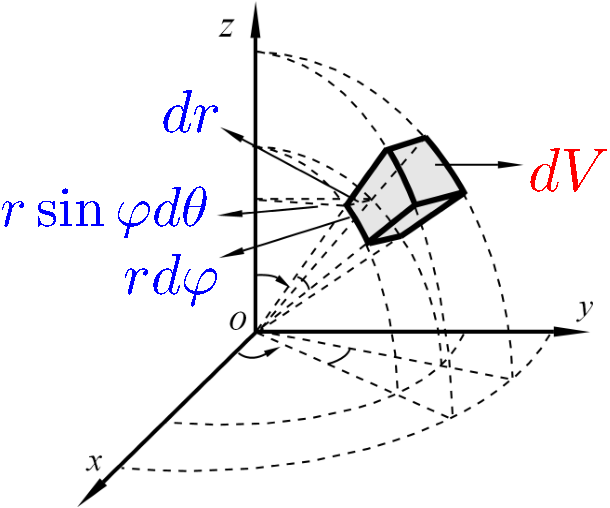
\includegraphics{./images/ch11/sphDv.pdf}}\pause 
			\end{center}
% 		\column{.4\textwidth}
			{\Large
			\vspace{-1em}
			$$\alert{\d V=r^2\sin\varphi \d r\d\theta \d\varphi}$$
			}
% 	\end{columns}
% 	$$\alert{\iiint_{\Omega}f(x,y,z)dV=\iiint_{\Omega}f(\rho\cos\theta,\rho\sin\theta,z)\rho
% 	d\rho d\theta dz}$$
\end{frame}

\begin{frame}
	\linespread{1.2}
	\begin{exampleblock}{{\bf 例8}\hfill}
		计算三重积分
		$$\iiint_{\Omega}(x^2+y^2+z^2)\d V,$$
		其中$\Omega$由$z=\sqrt{x^2+y^2}$与$x^2+y^2+z^2=R^2$所围成。
	\end{exampleblock}
\end{frame}

\begin{frame}
	\linespread{1.2}
	\begin{exampleblock}{{\bf 例9}\hfill}
		计算三重积分
		$$\iiint_{\Omega}(x^2+y^2)\d V,$$
		其中$\Omega$由$x^2+y^2+z^2=2az$与$x^2+y^2+z^2=2bz$所围成$(0<a<b)$。
	\end{exampleblock}
\end{frame}

\begin{frame}[<+->]{小结}
	\linespread{1.2}
	\ba{三重积分的计算}
	\begin{enumerate}
	  \item {\bf 柱坐标系:}
	  $$\d V=\rho \d\rho \d\theta \d z$$
	  \item {\bf 球坐标系:}
	  $$\d V=r^2\sin\varphi \d r\d\theta \d\varphi$$
	\end{enumerate}
	\pause \hrule
	\bigskip
	\centerline{\ba{根据被积函数和积分区域的特点灵活选择坐标系}}
\end{frame}

%=====================================
 
% \begin{frame}{title}
% 	\linespread{1.2}
% 	\begin{exampleblock}{{\bf title}\hfill}
% 		123
% 	\end{exampleblock}
% \end{frame}
% 
% \begin{frame}{title}
% 	\linespread{1.2}
% 	\begin{block}{{\bf title}\hfill}
% 		123
% 	\end{block}
% \end{frame}